\chapter{The Fundamental Group}

As we will see soon enough, the objects of the fundamental group are loops. So, we are going to make a group out of loops. A loop is nothing but a path with some base point. Now, it is a time to define a path.
\begin{definition}[\textbf{Path}]
Let $I=[0,1]$, the closed unit interval. A path from a point $a$ to a point $b$ in a topological space $X$ is a continuous function $f:I\rightarrow X$ with $f(0)=a$ and $f(1)=b$. Here $a$ and $b$ are called initial and terminal points respectively.
\end{definition}

\begin{figure}[hbt!]
\centering
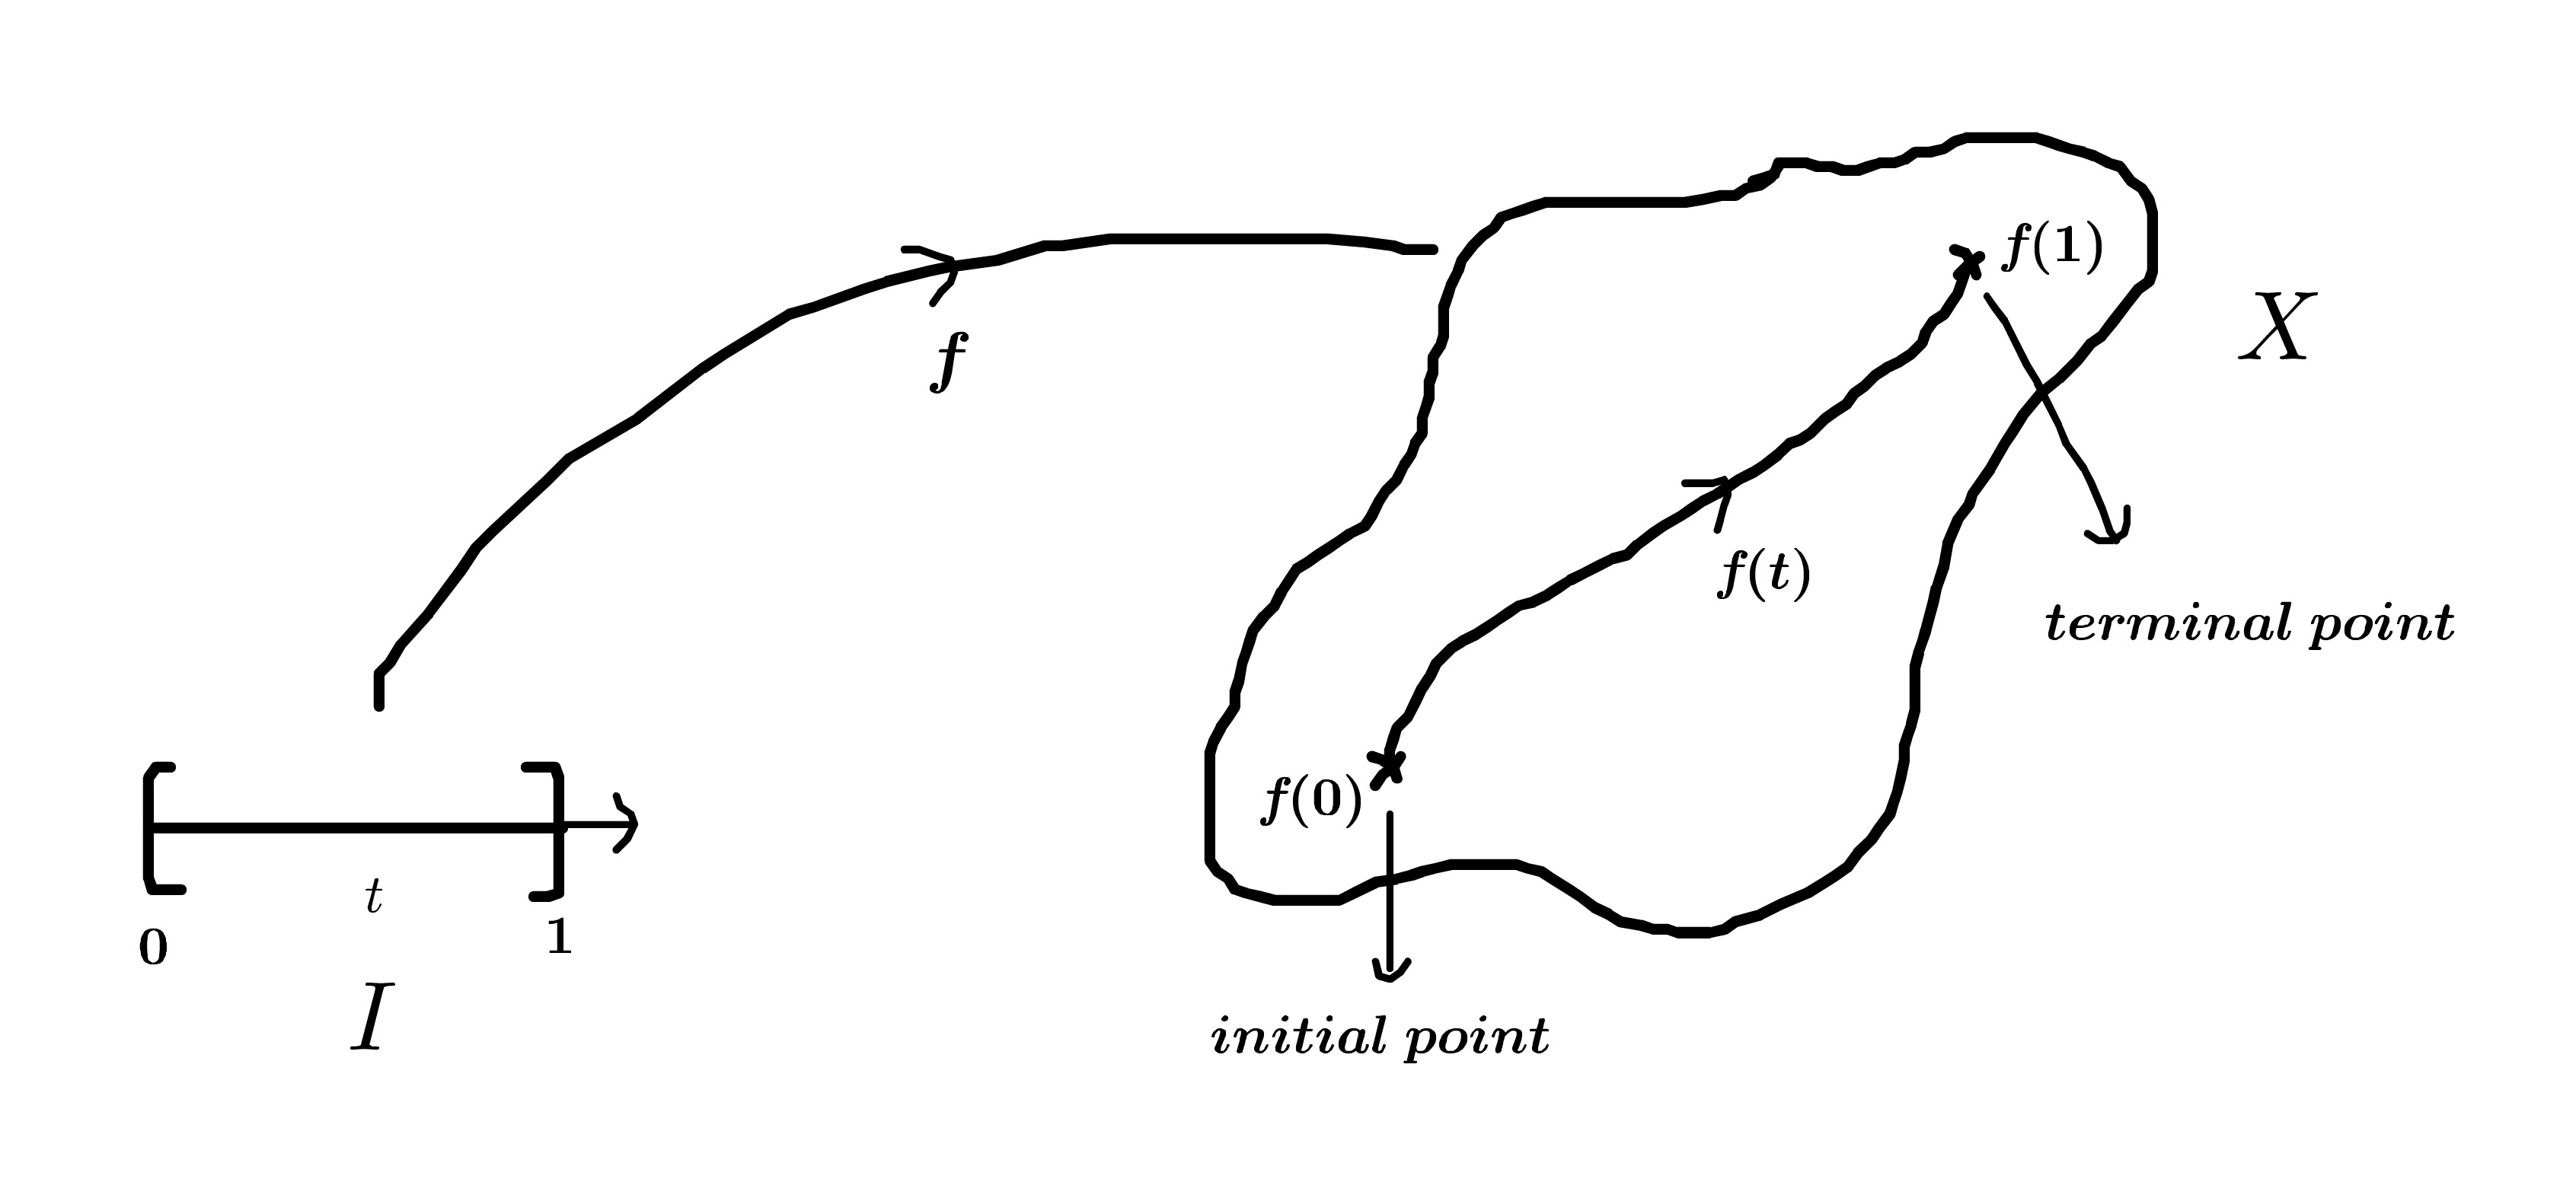
\includegraphics[width=.7\textwidth]{./images/path.jpg}
\caption{Path}
\end{figure}


\section{Homotopy}
\begin{definition}[\textbf{Homotopy}]
If $f$ and $f'$ are continuous maps of the space $X$ into the space $Y$, we say that $f$ is homotopic to $f'$ if there is a continuous map $F:X\times I \rightarrow Y$ such that
$$ F(x,0)=f(x) \qquad and \qquad F(x,1)=f'(x)$$
for each $x$. Where $I=[0,1]$ the unit interval. The map $F$ is called a \textbf{homotopy} between $f$ and $f'$. If $f$ is homotopic to $f'$ we write $f\simeq f'$. If $f\simeq f'$ and $f'$ is a constant map, we say that $f$ is \textbf{nulhomotopic}.
\end{definition}

We think of a homotopy as a continuous one-parameter family of maps from $X$ to $Y$. If we imagine the parameter $t$ as representing time, then the homotopy $F$ represents a continuous deforming of the map $f$ to the map $f'$, as $t$ goes from $0$ to $1$.

\section{Homotopy of Paths}
\begin{definition}
If $f:I\rightarrow X$ and $f':I\rightarrow X$ are two paths with the same initial point $p\in X$ and the same terminal point $q\in X$. We say that $f$ is homotopic to $f'$ if there is a continuous map $F$
$$
F: I\times I\rightarrow X \ni
$$

\begin{center}
$F(s,0)=f(s) \qquad$ and $\qquad F(s,1)=f'(s),$\\
$F(0,t)=p \qquad$ and $\qquad F(1,t)=q $
\end{center}

for each $s\in I$ and $t\in I$. We call $F$ a \textbf{path homotopy} between $f$ and $f'$ see figure \ref{path}. We denote $f\simeq_p f'$ to say $f$ is path homotopic to $f'$.
\end{definition}
\begin{figure}[hbt!]
\centering
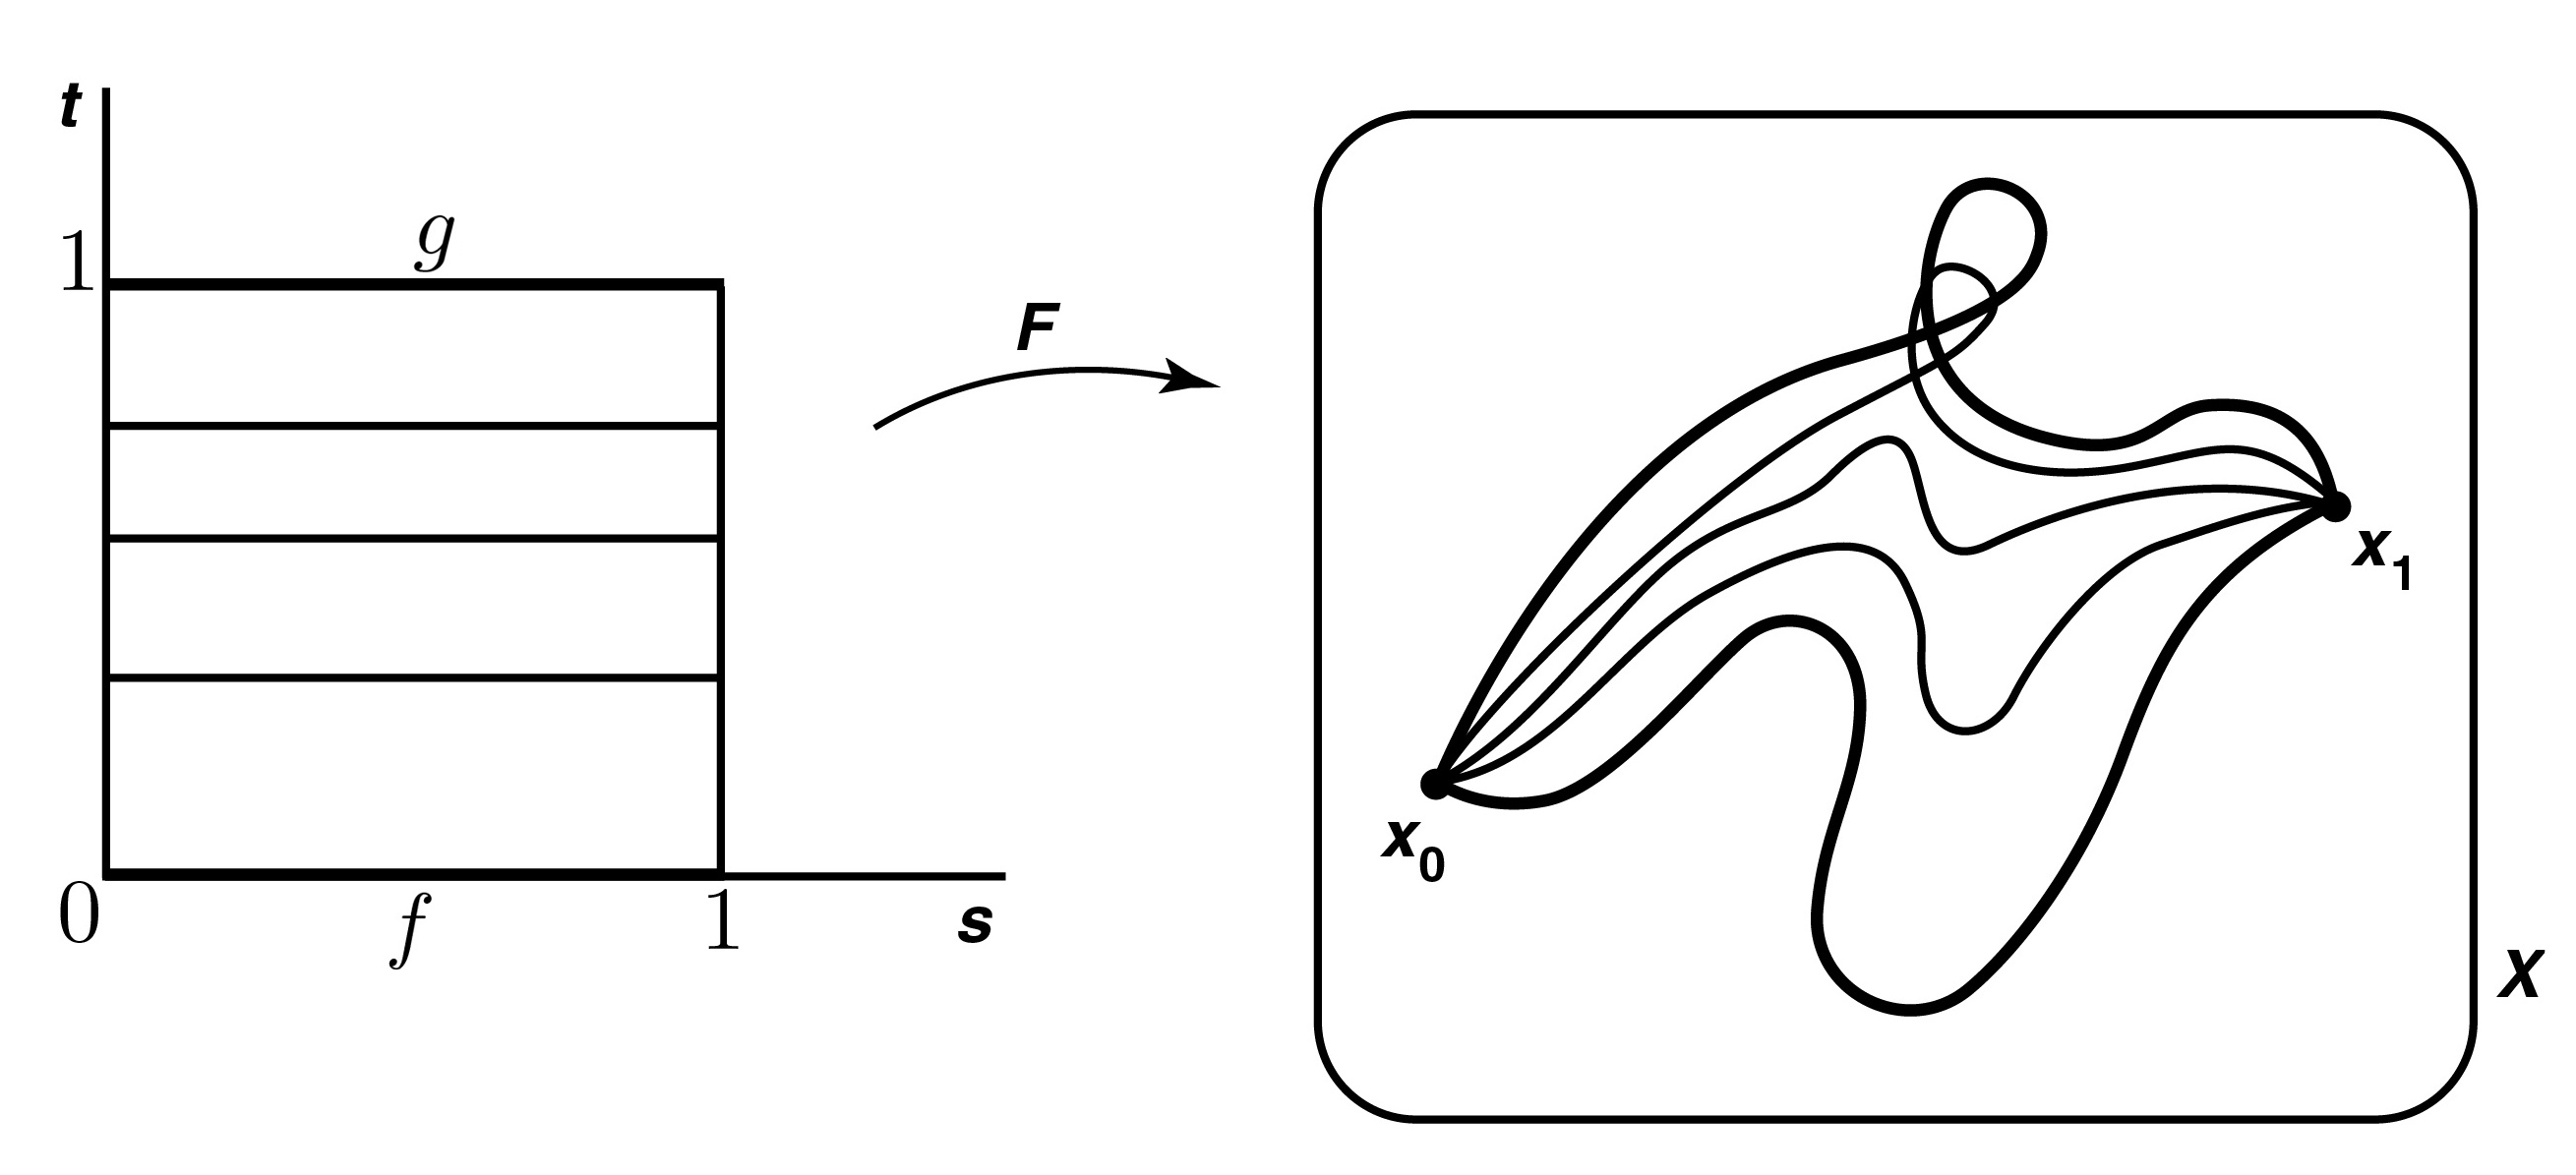
\includegraphics[width=.75\textwidth]{./images/def.jpg}
\caption{Homotopy of path}\label{path}
\end{figure}

\begin{prop}
The relations $\simeq$ and $\simeq_p$ are equivalence relations.
\end{prop}

\begin{proof}
(i) Given $f$ it is trivial that $f\simeq f$; the map $F(x,t)=f(x)$ is the required homotopy. If $f$ is a path, $F$ is a path homotopy.

(ii) Given $f\simeq f'$, we show that $f'\simeq f$. Let $F$ be a homotopy between $f$ and $f'$. Then $G(x,t)=F(x,1-t)$ is a homotopy between $f'$ and $f$. If $f$ a path homotopy  so is $G$.

(iii) Suppose that $f\simeq f'$ and $f'\simeq f''$. WTS $f\simeq f''$. Let $F$ be a homotopy between $f$ and $f''$ and let $F'$ be a homotopy between $f'$ and $f''$. Define $G:X\times I\rightarrow Y$ by the equation

$$
G(x,t)=
\begin{cases}
F(x,2t),&\mbox{ for }t\in[0,1/2]\\
F'(x,2t-1),&\mbox{ for }t\in[1/2,1]
\end{cases}
$$
The map $G$ is well-defined, since if $t=1/2$, we have
$$ F(x,2t)=f'(x)=F'(x,2t-1)$$
Because $G$ is continuous on the two closed subsets $X\times[0,1/2]$ and $X\times[1/2,1]$ of $X\times I$, it is continuous on all of $X\times I$, by pasting lemma (\ref{pasting}). Thus $G$ is the required homotopy between $f$ and $f"$.
\end{proof}
\medskip
The following figure illustrates if $F$ and $F'$ are path homotopies, so is $G$
\begin{figure}[hbt!]
\centering
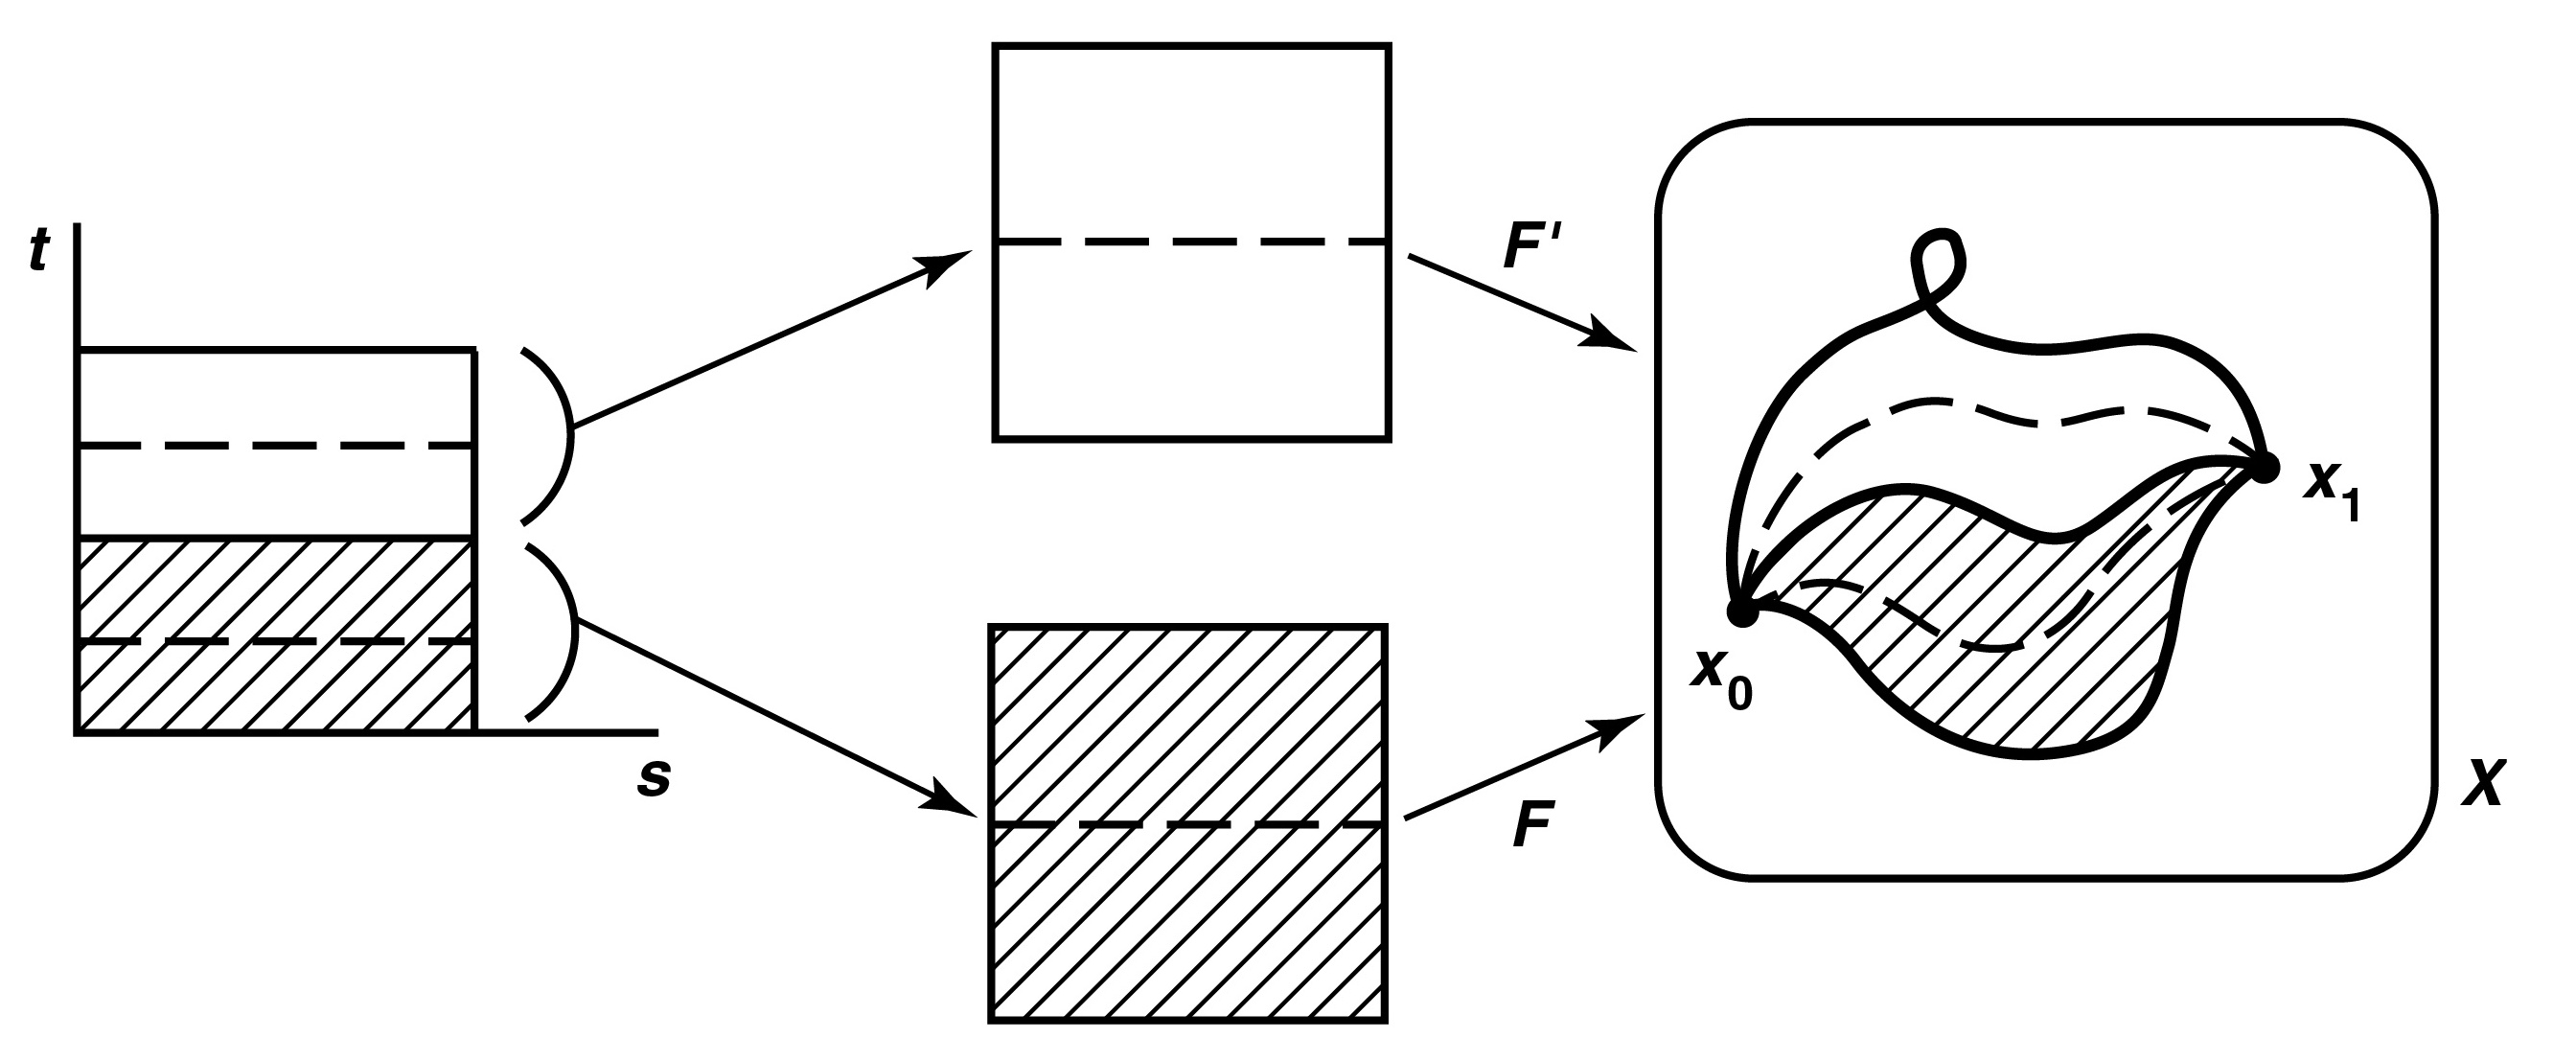
\includegraphics[width=.8\textwidth]{./images/equiv.jpg}
\caption{Transitive property of the homotopy}
\end{figure}


\begin{example}
Let $f$ and $g$ be any two continuous maps of space $X$ into $\mathbb{R}^2$ It is easy to see that $f$ and $g$ are homotopic; the map
$$
F(x,t)=(1-t)f(x)+tg(x)
$$
is a homotopy between them. It is called a straight-line homotopy because it moves the point $f(x)$ to the point $g(x)$ along the straight-line segment joining them.
\end{example}
\begin{prop}\label{homocomp}
If $h, h'$ are homotopic maps from $X$ into $Y$ and $k, k'$ are homotopic maps from $Y$ into $Z$ , then $k\circ h \simeq k' \circ h'$.
\end{prop}


\begin{proof}
Since $h\simeq h'$ there is a homotopy $H:X\times I \rightarrow Y$ with $H(s,0)=h(s),$ $H(s,1)=h'(s).$
Since $k\simeq k'$ there is a homotopy $K:Y\times I \rightarrow Z$ with $K(s,0)=k(s),$ $K(s,1)=kh'(s).$ Then define $F: X\times I\rightarrow Z$ by

$$
F(s,t)=
\begin{cases}
k(H(s,2t)),&0\leq t\leq 1/2\\
K(h'(s),2t-1),&1/2\leq t\leq 1
\end{cases}
$$
Then let's check that $F$ does what it ought to do, at different values of $t$.\\
\begin{align*}
t=0,\qquad F(s,o)=k(H(s,o))=k(h(s))=k\circ h(s)\\
t=1/2,\qquad F(s,1/2)=k(H(s,1))=k(h'(s))=k\circ h'(s)\\
\qquad \qquad F(s,1/2)=K(h'(s),0))=k(h'(s))=k\circ h'(s)\\
t=1,\qquad F(s,1)=K(h'(s),1)=k'(h'(s))=k'\circ h'(s)
\end{align*}
Thus $F$ is the desired homotopy.
\end{proof}


\begin{definition}
A constant path in a topological space $Y$ is a constant function from $I$ into $Y$. i.e. $f:I\rightarrow Y$ is a constant path if there is $y_0\in Y$ such that $f(s)=y_0$ for all $s\in I$.
\end{definition}

\begin{definition}
Two topological spaces $X$ $\&$ $Y$ are said to be homotopy equivalent or of the \textbf{same same homotopy} type if there exist a continuous maps $f:X\rightarrow Y$ and $g:Y\rightarrow X$ such that $g\circ f $ is homotopic to the identity map $id_X$ and $f\circ g\simeq id_Y$.
\end{definition}




Homeomorphic spaces are of the same homotopy type. To show this let $X$ and $Y$ be homeomorphic spaces. Then there exists a continuous map $f:X\rightarrow Y$ with a continuous inverse $f^{-1}:Y\rightarrow X$. Thus $f\circ f^{-1}=id_Y$ and $f^{-1}\circ f=id_X$. Since homotopy is an equivalence relation this implies $f\circ f^{-1}\simeq id_Y$ and $f^{-1}\circ f\simeq id_X$  Q.E.D. But the converse is not true: for example, a solid disk is not homeomorphic to a single point (since there is no bijection between them), although the disk and the point are homotopy equivalent (since you can deform the disk along radial lines continuously to a single point). Spaces that are homotopy equivalent to a point are called contractible.

\begin{prop}
Same homotopy type is an equivalence relation on the collection of topological space.
\end{prop}

\begin{proof}
\begin{description}
  \item[Reflexive:] Let $X$ be a topological space. Define $id:X\rightarrow X$ by $id(x)=x.$
  \item[Symmetric:] Let $X $ and $Y$ are spaces of the same homotopy. Then there exist a continuous maps $f:X\rightarrow Y$ and $g:Y\rightarrow X$ such that $g\circ f $ is homotopic to the identity map $id_X$ and $f\circ g\simeq id_Y$. Thus $Y$ and $X$ are of the same homotopy.
  \item[Transitive:] Suppose $X $ and $Y$ are spaces of the same homotopy. Then there exist a continuous maps $f_1:X\rightarrow Y$ and $g_1:Y\rightarrow X$ such that $g_1\circ f_1 \simeq id_X$ and $f_1\circ g_1\simeq id_Y$. Similarly, if $Y $ and $Z$ are spaces of the same homotopy, then there exist a continuous maps $f_2:Y\rightarrow Z$ and $g_2:Z\rightarrow Y$ such that $g_2\circ f_2 \simeq id_Y$ and $f_2\circ g_2\simeq id_Z$. WTS $(g_1\circ g_2)\circ(f_2\circ f_1)\simeq id_X$ and $(f_2\circ f_1)\circ(g_1\circ g_2)\simeq id_Z$. Now
   $$(g_1\circ g_2)\circ(f_2\circ f_1)=g_1\circ \underbrace{(g_2\circ f_2)\circ f_1 \simeq g_1\circ (id_Y)}_{\Delta_1}\circ f_1= g_1\circ f_1\simeq id_X.$$
Similarly, $$(f_2\circ f_1)\circ(g_1\circ g_2)=f_2\circ \underbrace{(f_1\circ g_1)\circ g_2 \simeq f_2\circ (id_Y)}_{\Delta_2}\circ g_2= f_2\circ g_2\simeq id_Z.$$
\end{description}
The steps $\Delta_1$ and $\Delta_2$ are actually true by proposition (\ref{homocomp}).
\end{proof}

\medskip
\begin{definition}[\textbf{Concatenation}]
If $f$ is a path in $X$ from $x_0$ to $x_1$, and if $g$ is a path from $x_1$ to $x_2$, we define the \textbf{product} of $f\ast g$ of $f$ and $g$ to be the path $h$ given by the equations
$$
h(s)=
\begin{cases}
f(2s),&\mbox{ for }s\in[0,1/2]\\
g(2s-1),&\mbox{ for }s\in[1/2,1]
\end{cases}
$$
\end{definition}
The function $h$ is well-defined and continuous, by the pasting lemma (\ref{pasting}); it is a path in $X$ from $x_0$ to $x_2$. We think of $h$ as the path whose first half is the path $f$ and whose second half is the path $g$.
The product operation on paths induces a well-defined operation on path-homotopy classes, defined by the equation
$$[ f ] \ast [g] = [ f \ast g].$$
To verify this fact, let $F$ be a path homotopy between $f$ and $f'$ and let $G$ be a path homotopy between $g$ and $g'$. Define
$$
H(s,t)=
\begin{cases}
F(2s,t),&\mbox{ for }s\in[0,1/2]\\
G(2s-1,t),&\mbox{ for }s\in[1/2,1]
\end{cases}
$$
Because $F(1, t) = x_1 = G(0, t)$ for all $t$, the map $H$ is well-defined; it is continuous by the pasting lemma (\ref{pasting}).


\section{The Fundamental Group}

\begin{definition}
A loop in a topological space is a path in the space whose initial point and terminal point are the same. If the initial point and terminal point of a loop in the topological space $X$ are both the point $x_0\in X$, we will say that the loop is based at $x_0$.
\end{definition}

Let $X$ be a topological space and $x_0$ be a point in $X$. Then the $x_0$ neighborhood of curves in $X$, $C(X,x_0)$, is the collection of all continuous mappings $f:I\rightarrow X$ of the unit interval into $X$ such that $f(0)=x_0=f(1)$. i.e. the collection of all loops based at $x_0$.


\begin{definition}
Let $f$ and $g$ be two maps in $C(X,x_0)$ that means $f$ and $g$ are loops based at $x_0$. Then $f$ is homotopic to $g~modulo~x_0$ if $f$ and $g$ are homotopic in a usual sense with some additional restriction. Here is the restriction: If H is the homotopy between $f$ and $g$ , then $H(0,t)=x_0=H(1,t)$.
\end{definition}

\begin{theorem}
The set of path homotopy equivalence class of loops based at $x_0\in X$ is a group under the ''multiplication'' defined by $[\alpha][\beta]=[\alpha\beta]$. This group is denoted by $\pi_1(X,x_0)$ and is called the fundamental group of $X$ at $x_0$.
\end{theorem}
\begin{proof}
WTS that the four group axioms are satisfied here.
\begin{description}
  \item[I.] Our first task is to show the ''multiplication'' is well-defined. Thus we have to show that it is independent of what representatives $\alpha$ and $\beta$ of $[\alpha]$ and $[\beta]$ are used. This done by proving if $\alpha_1\simeq \alpha_2$ ,$\beta_1\simeq\beta_2$ then $\alpha_1\beta_1\simeq\alpha_2\beta_2$. To show this let $H_1$ and $H_2$ be homotopies such that
      $$ H_1(s,0)=\alpha_1(s), H_1(s,1)=\alpha_2(s), \qquad H_1(0,t)=x_0=H_1(1,t)$$
      $$ H_2(s,0)=\beta_1(s), H_2(s,1)=\beta_2(s), \qquad H_2(0,t)=x_0=H_2(1,t)$$
  Define
$$
H(s,t)=
\begin{cases}
H_1(2s,t),&\mbox{ for }s\in[0,1/2]\\
H_2(2s-1,t),&\mbox{ for }s\in[1/2,1]
\end{cases}
$$
The mapping $H$ is well-defined and it is continuous by pasting lemma. Also
\[
    H(s,0) = \left\{\begin{array}{lr}
        H_1(2s,0)=\alpha_1(2s), & \text{ for }\ 0\leq s\leq 1/2\\
        H_2(2s-1,0)=\beta_1(2s-1), & \text{ for }\ 1/2\leq s\leq 1
        \end{array}\right\} = (\alpha_1\ast\beta_1)(s)
\]
and
\[
    H(s,1) = \left\{\begin{array}{lr}
        H_1(2s,1)=\alpha_2(2s), & \text{ for }\ 0\leq s\leq 1/2\\
        H_2(2s-1,1)=\beta_2(2s-1), & \text{ for }\ 1/2\leq s\leq 1
        \end{array}\right\} = (\alpha_2\ast\beta_2)(s)
\]
Thus $\pi_1(X,x_0)$ is closed under this operation.
  \item[II.] The associative property follows if we can show that $(\alpha \ast \beta)\ast\gamma \simeq\alpha(\beta\ast\gamma)$

  From the definition
$$
[(\alpha\ast\beta)\ast\gamma](s)=
\begin{cases}
\alpha(4s),&\mbox{ for }\ 0\leq s\leq 1/4\\
\beta(4s-1),&\mbox{ for }\ 1/4\leq s\leq 1/2\\
\gamma(2s-1)&\mbox{ for }\ 1/2\leq s\leq 1\\
\end{cases}
$$
and
$$
[\alpha\ast(\beta\ast\gamma)](s)=
\begin{cases}
\alpha(2s),&\mbox{ for }\ 0\leq s\leq 1/2\\
\beta(4s-2),&\mbox{ for }\ 1/2\leq s\leq 3/4\\
\gamma(4s-3)&\mbox{ for }\ 3/4\leq s\leq 1\\
\end{cases}
$$
A homotopy $H$ between these two mappings may be given as follows
$$
H(s,t)=
\begin{cases}
\alpha(\frac{4s}{t+1}),&\mbox{ for }\ t\geq 4s-1\\
\beta(4s-t-1),&\mbox{ for }\ 4s-1\geq t\geq 4s-2\\
\gamma(\frac{4s-t-2}{2-t})&\mbox{ for }\ 4s-2\geq t\\
\end{cases}
$$
We can use the following diagram to obtain the above homotopy

\begin{figure}[hbt!]
\centering
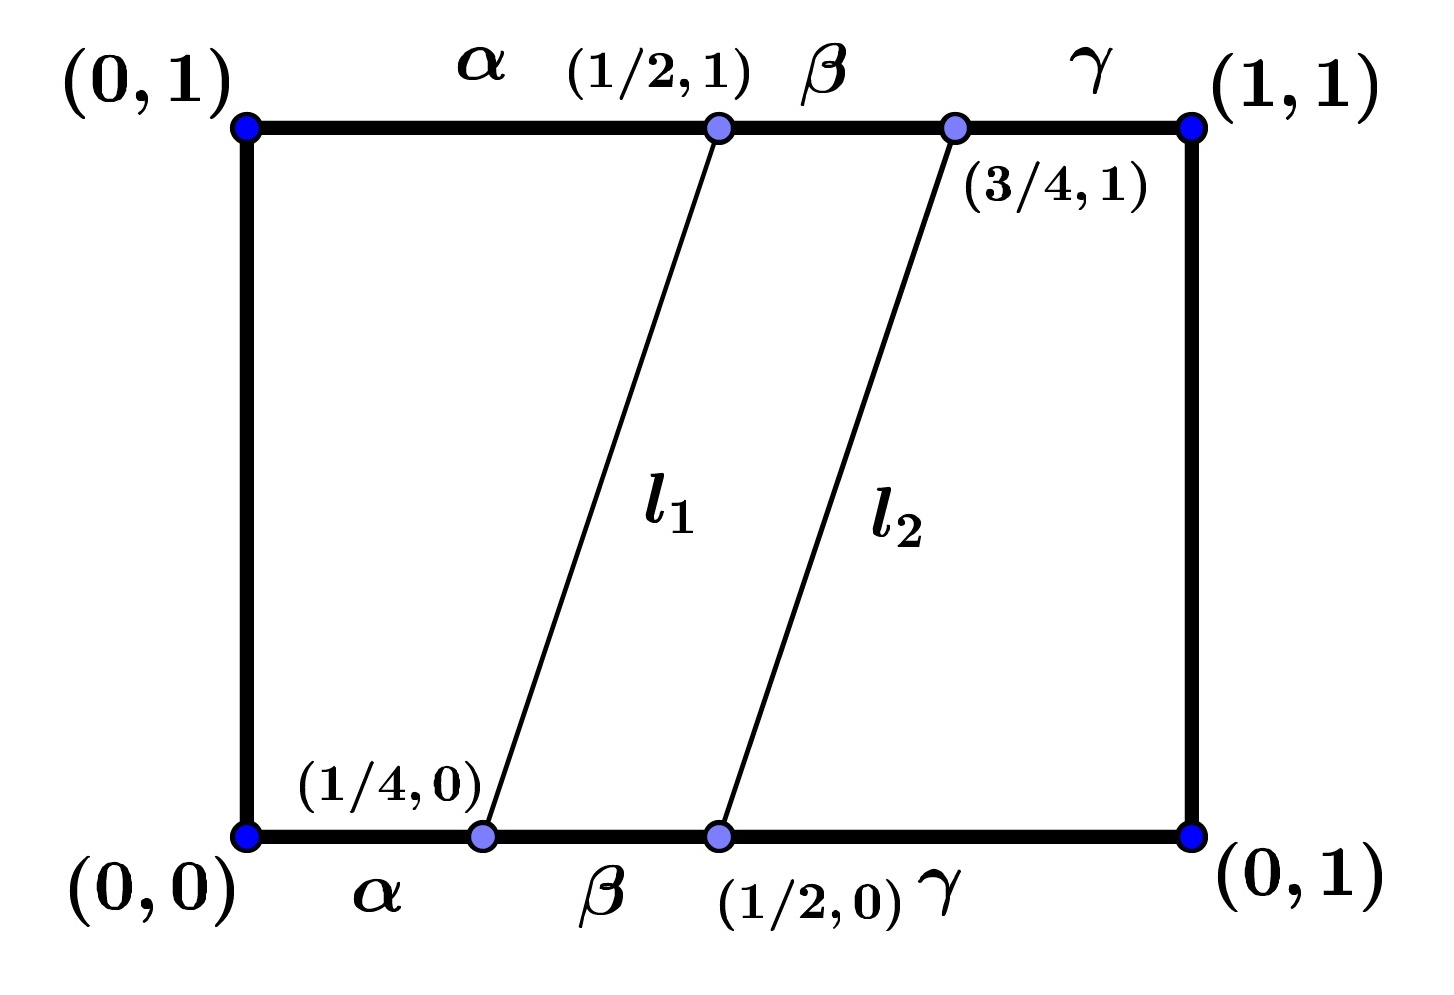
\includegraphics[width=.6\textwidth]{./images/Asso.jpg}
\caption{Associativity property}
\end{figure}

To check that $H$ is the desired homotopy

\[
H(s,0)=\left\{\begin{array}{lr}
\alpha(4s),&\text{for}\ 0\geq 4s-1 \text{ or } 0\leq s\leq1/4 \\
\beta(4s-1),&\mbox{ for }\ 4s-1\geq 0\geq 4s-2 \text{ or } 1/4\leq s\leq1/2\\
\gamma(2s-1)&\mbox{ for }\ 4s-2\geq 0 \text{ or } 1/2\leq s\leq1
\end{array}\right\}=(\alpha\ast\beta)\ast\gamma
\]

and

\[
H(s,1)=\left\{\begin{array}{lr}
\alpha(2s),&\text{for}\ 1\geq 4s-1 \text{ or } 0\leq s\leq1/2\\
\beta(4s-2),&\mbox{ for }\ 4s-1\geq 1\geq 4s-2 \text{ or } 1/2\leq s\leq 3/4\\
\gamma(4s-3)&\mbox{ for }\ 4s-2\geq 1 \text{ or } 3/4\leq s\leq 1
\end{array}\right\}=\alpha\ast(\beta\ast\gamma)
\]
Hence associativity.
  \item[III.] The existence of an identity.

Let $e_{x_0}$ denote the constant mapping $e_{x_0}(x)=x_0$ for all $x\in I$. We claim the equivalence class $[e_{x_0}]$ is the identity element of $\pi_1(X,x_0)$. To prove this it suffices to show that $\alpha\ast e_{x_0}$ for any function in $C(X,x_0)$. This is done by constructing the homotopy
$$
H(s,t)=
\begin{cases}
\alpha(\frac{2s}{1+t}),&\mbox{ for }\ t\geq 2s-1\\
x_0,&\mbox{ for }\  t\leq 2s-1
\end{cases}
$$
The continuity of $H$ is in question where $t=2s-1$, but for any such point $H(s,t)=x_0$, so $H$ is continuous as required. A check at the boundary conditions shows that
\[ H(s,0) = \left\{\begin{array}{lr}
        \alpha(2s) & \text{ for }\ 0\ge 2s-1 \text{ or } 0\leq s\leq 1/2 \\
        x_0 & \text{ for }\ 0\leq 2s-1 \text{ or } 1/2\leq s\leq 1
        \end{array}\right\} = \alpha\ast e_{x_0}
\]
and $H(s,1)=\alpha(s) \text{ for } 1\ge 2s-1 \text{ or } 0\leq s\leq 1.$
  \item[IV.] The existence of inverse element.

  To show this let $\alpha$ be any mapping in $C(X,x_0)$ and define a new mapping $\alpha^{-1}$ by setting
  $$\alpha^{-1}(s)=\alpha(1-s)$$
  Thus, $\alpha^{-1}(0)=\alpha(1)=\alpha^{-1}(1)=\alpha(0),$ so $\alpha^{-1}$ is an element of $C(X,x_0)$. We want to show $\alpha\ast\alpha^{-1}\simeq e_{x_0}$. By definition
$$
(\alpha\ast\alpha^{-1})(s)=
\begin{cases}
\alpha(2s),&\mbox{ for }\ 0\leq s\leq 1/2\\
\alpha^{-1}(2s-1)=\alpha(2-2s),&\mbox{ for }\  1/2\leq s\leq1
\end{cases}
$$
Now, we construct a homotopy between $\alpha\ast\alpha^{-1}$ and $e_{x_0}$ by setting
$$
H(s,t)=
\begin{cases}
\alpha(\frac{2s}{1-t}), & \text{for }t\geq 2s-1, 0\leq s\leq 1/2\\
        x_0,  & \text{for } t\geq 1-2s, 0\leq s\leq 1/2 ;\\
                               & t\geq 2s-1, 1/2\leq s\leq 1\\
       \alpha(\frac{2s-2}{t-1}), & \text{for } t\leq 2s-1, 1/2\leq s \leq 1
\end{cases}
$$
To check the continuity of $H$, at $t=1-2s$
$$ H(s,t)=\alpha\biggl(\frac{2s}{1-(1-2s)}\biggl)=\alpha(1)=x_0$$
And for $t=2s-1$
$$ H(s,t)=\alpha\biggl(\frac{2s-2}{2s-1-1}\biggl)=\alpha(1)=x_0$$
Hence $H$ has the necessary continuity. Checking the boundary conditions
\[ H(s,0) = \left\{\begin{array}{lr}
        \alpha(2s) & \text{ for }\ 0\leq 1-2s \text{ or } 0\leq s\leq 1/2 \\
        x_0 & \text{ for }\ 2s-1\leq0\leq1-2s \text{ or }  s\leq 1/2\\
        \alpha(\frac{2s-2}{-1})=\alpha(2-2s) & \text{ for }\ 0\leq 2s-1 \text{ or } 1/2\leq s\leq 1
        \end{array}\right\} = \alpha\ast \alpha^{-1}
\]
And $H(s,1)=x_0=e_{x_0}$
This shows that the class $[f^{-1}]$ is the inverse of $[f]$.
\end{description}
This completes the proof that $\pi_1(X,x_0)$ is a group, the fundamental group of $X$ based at $x_0$.
\end{proof}

Instead of the fundamental group of $X$ based at $x_0$ it would be nice to have the fundamental group of $X$. In other words, we would like to have the fundamental group depend only on the space, and not on the particular point of the space that we base our loops at.

\medskip
\begin{thm}

Let $x_0,x_1\in X$. If there is a path in $X$ from $x_0$ to $x_1$ then the groups $\pi_1(X,x_0)$ and $\pi_1(X,x_1)$ are isomorphic.

\end{thm}

\begin{proof}
To show the two groups are isomorphic is just a matter of finding a bijective map from one to the other.

Let $\gamma$ be a path from $x_0$ to $x_1$. If $\alpha$ is a loop based at $x_0$, then $(\gamma^{-1}\ast\alpha)\ast \gamma $ is a closed path based at $x_1$.

\begin{figure}[hbt!]
\centering
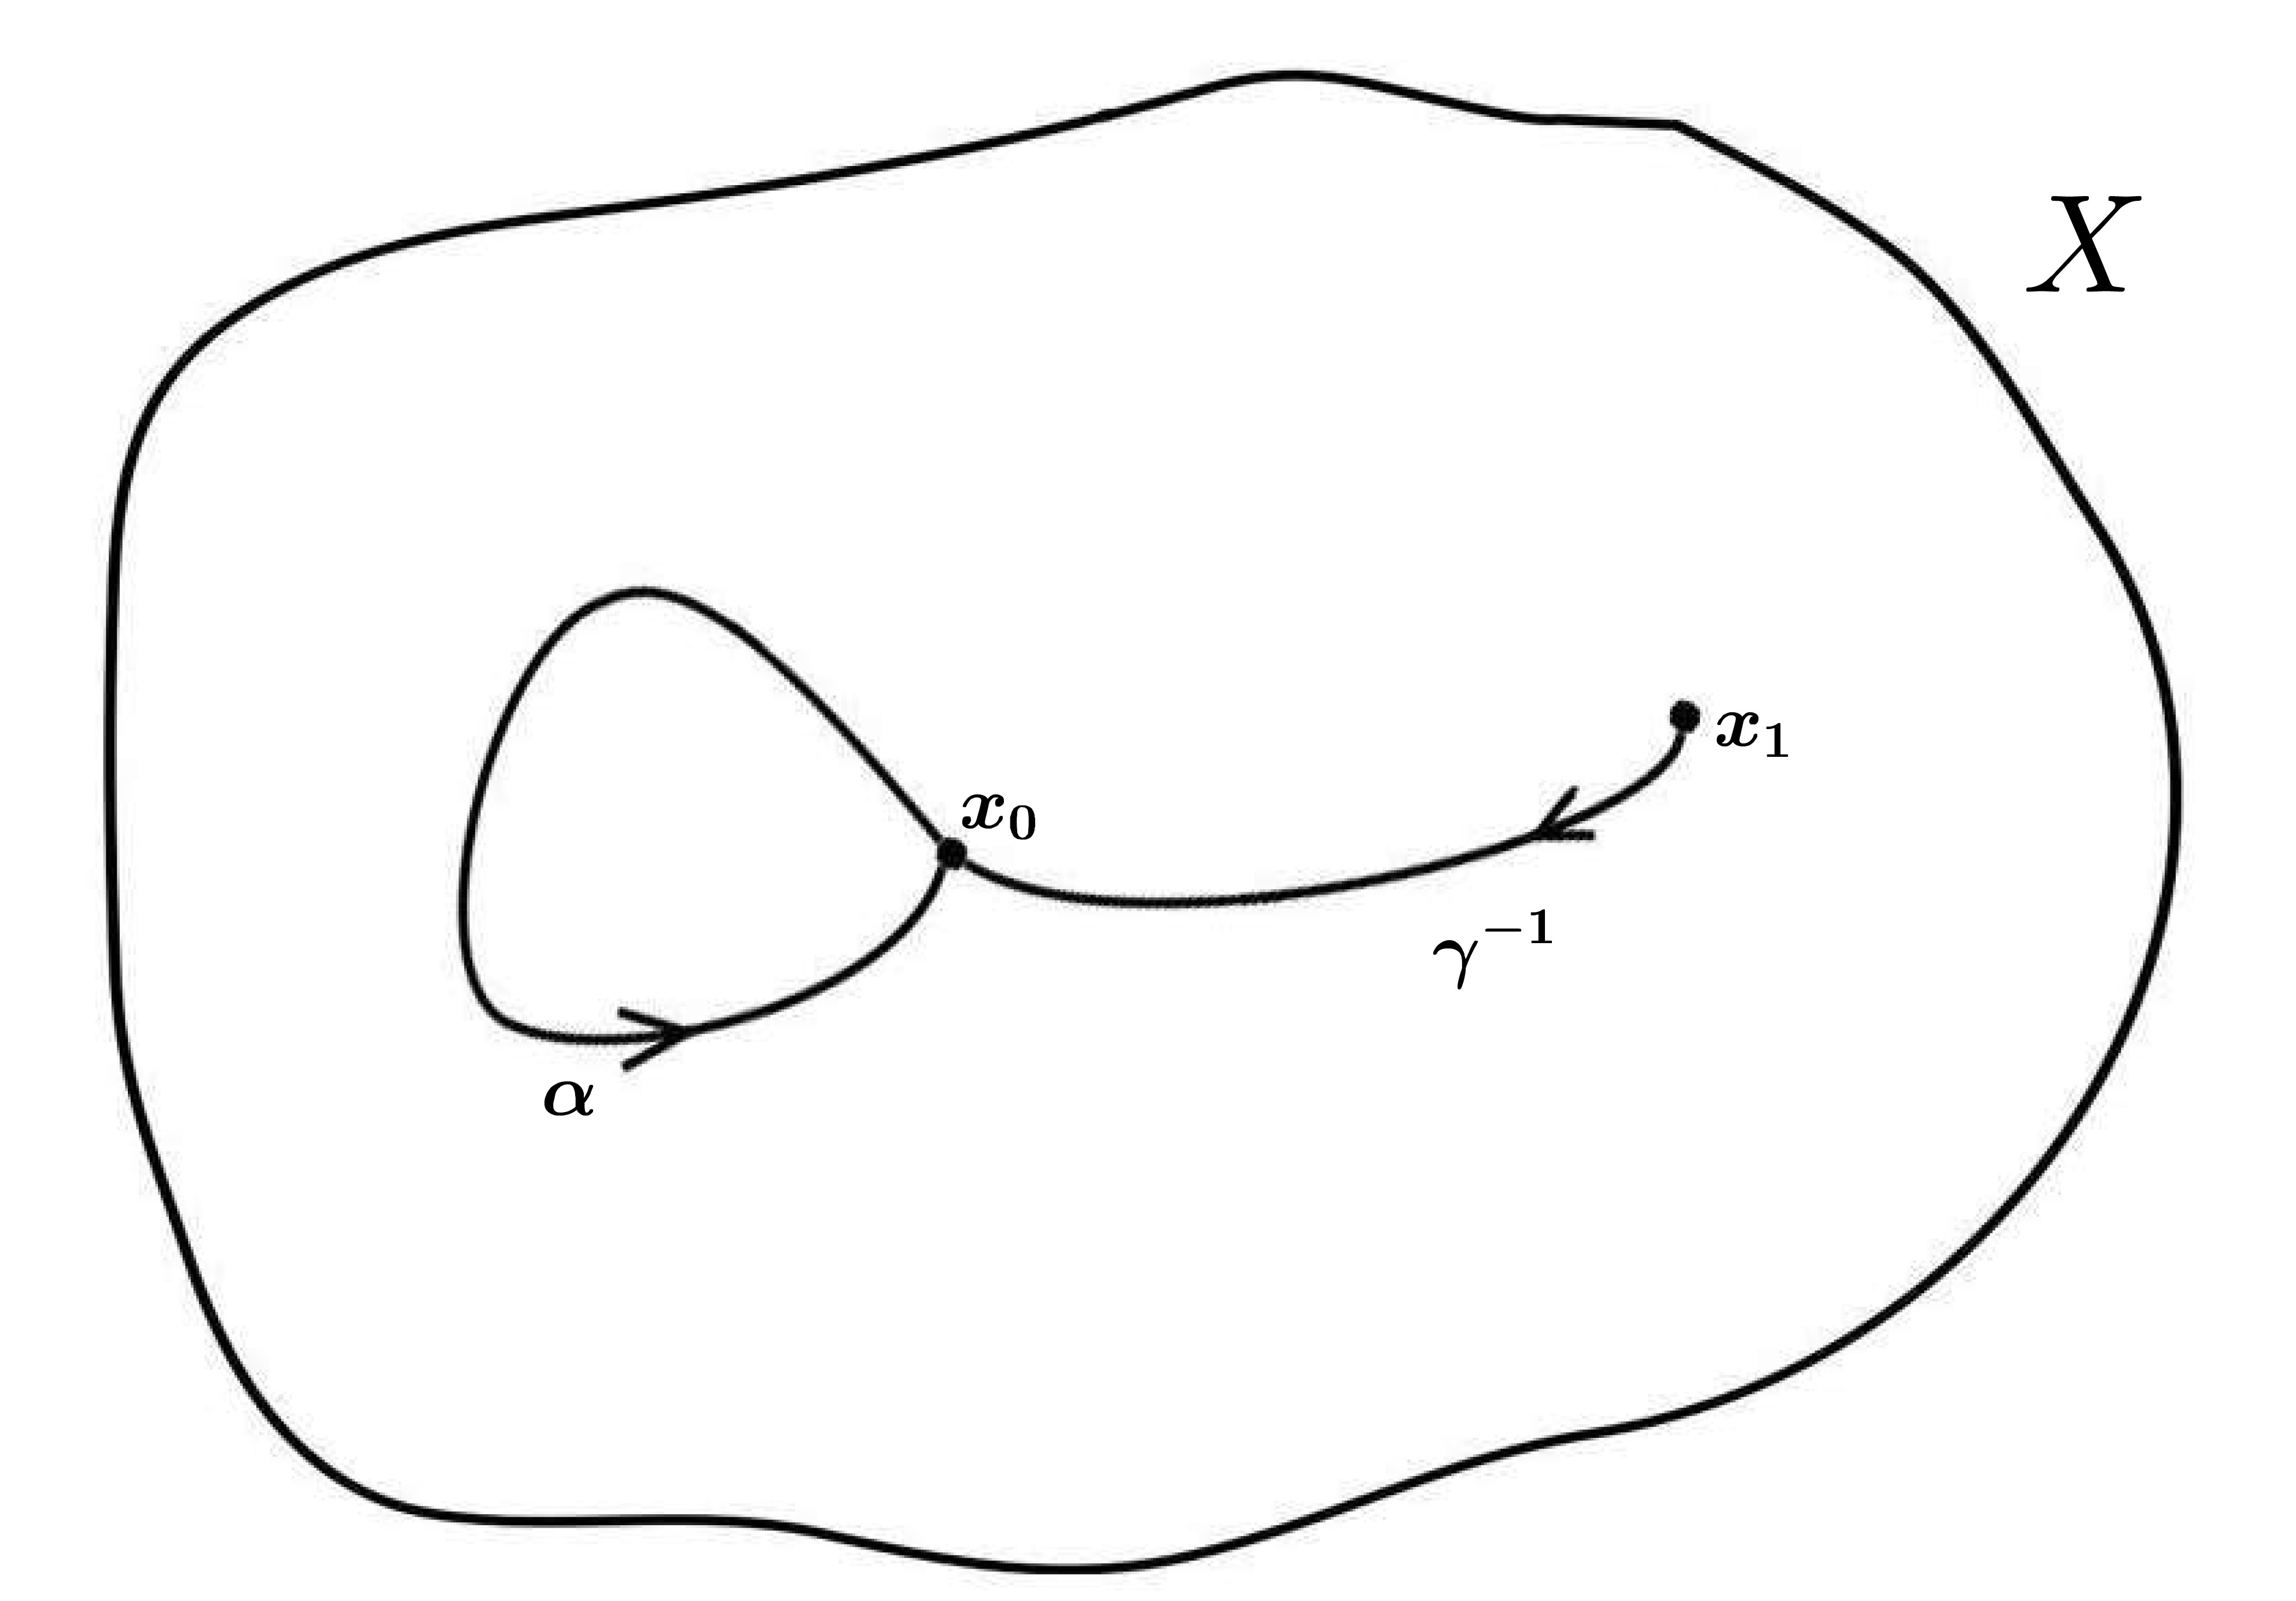
\includegraphics[width=.45\textwidth]{./images/loop.jpg}
\caption{The importance of base point}
\end{figure}



We therefore define $$ u_\gamma:\pi_1(X,x_0)\rightarrow \pi_1(X,x_1)  $$
by $u_\gamma[\alpha]=[\gamma^{-1}\ast\alpha\ast\gamma]$ that is, follow $\gamma^{-1}$ from $x_1$ to $x_0$, then follow $\alpha$ around back to $x_o$, then follow $\gamma$ back to $x_1$, all giving a loop based at $x_1$.
\begin{align*}
u_\gamma([\alpha]\ast[\beta])&=u_\gamma([\alpha\ast\beta])\\
                             &=[\gamma^{-1}\ast\alpha\ast\beta\ast\gamma]\\
                             &=[\gamma^{-1}\ast\alpha\ast\gamma\ast\gamma^{-1}\ast\beta\ast\gamma]\\
                             &=[\gamma^{-1}\ast\alpha\ast\gamma]\ast[\gamma^{-1}\ast\beta\ast\gamma]\\
                             &=u_\gamma([\alpha])\ast u_\gamma([\beta])
\end{align*}
Thus, $u_\gamma$ is a homomorphism.

Using the path $\gamma^{-1}$ from $x_1$ to $x_0$ we can define

$$u_{\gamma^{-1}}: \pi_1(X,x_1)\rightarrow \pi_1(X,x_0)$$

by $u_{\gamma^{-1}}([\alpha])=[\gamma\ast\alpha\ast\gamma^{-1}]$.\\
Now, check \begin{align*}
u_{\gamma^{-1}}u_\gamma[\alpha]=u_{\gamma^{-1}}[\gamma^{-1}\ast\alpha\ast\gamma]=[\gamma\ast\gamma^{-1}\ast\alpha\ast\gamma\ast\gamma^{-1}]=[\alpha]\\
u_{\gamma}u_{\gamma^{-1}}[\alpha]=u_{\gamma}[\gamma\ast\alpha\ast\gamma^{-1}]=[\gamma^{-1}\ast\gamma\ast\alpha\ast\gamma^{-1}\ast\gamma]=[\alpha]
\end{align*}
So, $u_\gamma$ is bijective and hence an isomorphism.
\end{proof}

\begin{definition}
A space $X$ is said to be path connected if any two points of $X$ can be joined by a path in $X$.
\end{definition}

\begin{cor}
If $X$ is a path connected space, then $\pi_1(X,x_0)$ and $\pi_1(X,x_1)$ are isomorphic groups for any pair of points $x_0,x_1\in X$.
\end{cor}

Let's look at some examples and wind up our discussion

\begin{example}
(\textbf{A simple connected space})

Suppose that a topological space $X$ is simply connected. In this case all loops with a base point $x_0$ are homotopic, resulting in one equivalence class. The result is $\pi_1(X)=0$, which is a group that consists of only the identity element.
\end{example}

\begin{example}
(\textbf{Circle})

Suppose $X=\mathbb{S}^1$. In this case there is an equivalence class for each $i\in \mathbb{Z}$, the set of integers. If $i\ge0$, then it means that the path travels $i$ times around $\mathbb{S}^1$ in the counterclockwise direction and then returns to $x_0$. If $i\le0$, then the path travels around $i$ times in in the clockwise direction. If $i=0$, then the path is equivalent to the one that remain at $x_0$ (constant loop). The fundamental group is $\mathbb{Z}$ with respect to the operation addition. If $\alpha_1$ travels $i_1$ times counterclockwise and $\alpha_2$ travels $i_2$ times counterclockwise, then $\alpha =\alpha_1\circ\alpha_2$ belongs to the class of loops that travel around $i_1+i_2$ times counterclockwise.

Consider additive inverses. If a path travels seven times around $\mathbb{S}^1$, and it is combined with a path that travels seven times in the opposite direction, the result is homotopic to the constant path (a path that remains at $x_0$). Thus, $\pi_1(\mathbb{S}^1)=\mathbb{Z}$.
\end{example}
Determining whether two given topological spaces are homeomorphic is a fundamental question in topology.

Showing two space are homeomorphic is a matter of constructing a continuous map from one to the other which has also a continuous inverse.

If we can find some topological property that holds for one topological space but not for the other, then this two spaces are not homeomorphic.

\begin{example}
(1) $[0,1]$ is not homeomorphic to $(0,1)$ since the first is compact and the second is not.
(2) $\mathbb{R}$ is not homeomorphic to $\mathbb{R}^2$ since deleting a point from $\mathbb{R}^2$ leaves a connected space and deleting a point from $\mathbb{R}$ does not.
(3) [i.] $\mathbb{R}^2$ is not homeomorphic to $\mathbb{R}^3$. Because deleting a point from $\mathbb{R}^3$ leaves a simply connected space, but deleting a point from $\mathbb{R}^2$ does not. [ii.] $S^2\ncong T$ using similar argument.
        
\end{example}
As we have seen earlier, the idea of \textbf{simple connectedness} is generalised through the \textbf{fundamental group}, which includes simple connectedness as a special case.
The condition of simple connectedness is just the condition that the fundamental group of $X$ is the trivial group.
So, the most important way of determining two spaces are not homeomorphic is by using their fundamental group.